\subsubsection{Experiments for Eliciting Calm Emotion}

To elicit the emotional state of calmness across three intensities, participants were exposed to video and audio stimuli known to promote relaxation. These tasks include a combination of soothing visual elements, relaxing music, and breathing techniques that are widely used in stress reduction and mindfulness practices.

\paragraph*{Low-Intensity Calmness – Rain and Relaxing Music Video}

The first task aimed at inducing a low level of calmness involved watching a video featuring soft rain visuals accompanied by relaxing ambient music (\url{https://youtu.be/PjUZbgZfMOo}) \citep{jm_professor_relaxing_music}. This combination is often used in meditative settings and is known for its ability to promote mild tranquility.

Research indicates that auditory stimuli such as slow-tempo, gentle music, when paired with natural sounds like rainfall, can work synergistically to reduce physiological arousal and promote emotional relaxation. These types of stimuli are frequently used in guided meditations and background soundtracks for relaxation, reflecting their general effectiveness in inducing calmness at a subtle level.

\paragraph*{Medium-Intensity Calmness – Music with Guided Breathing Exercise}

The second task combines relaxing music with a breathing exercise guided through video (\url{https://youtu.be/uxayUBd6T7M}) \citep{calm2020breathe}. This task requires the participant to actively engage in slow, deep breathing synchronized with musical rhythm, which helps regulate physiological responses and reduce stress.

Scientific evidence supports the role of deep breathing in stimulating the parasympathetic nervous system and lowering stress levels. When breathing is consciously controlled and paired with soothing music, it can lead to a more focused and deeper relaxation experience than passive listening alone. This form of active engagement is shown to promote a stronger state of calmness by influencing heart rate variability and promoting emotional self-regulation.

\paragraph*{High-Intensity Calmness – Listening to “Weightless” by Marconi Union}

For high-intensity calmness, participants listened to the song “Weightless” by Marconi Union while watching its official visual accompaniment (\url{https://youtu.be/UfcAVejslrU}) \citep{justmusictv2015weightless}. This song has been labeled as “the world’s most relaxing song” and has been scientifically validated for its profound impact on stress and anxiety levels.

Studies have reported that listening to “Weightless” can reduce anxiety by up to 65\% and lower physiological resting states by up to 35\%~\citep{cooper2011study}. The song was developed in collaboration with sound therapists, featuring a gradually slowing tempo from 60 to 50 beats per minute, low-frequency tones, and ambient instrumentation including piano, guitar, chimes, and subtle vocals.

Comparative studies suggest that listening to this track can be more relaxing than receiving a massage, and in some cases, it has shown effects comparable to anxiety medications~\citep{psychologytoday_weightless}. These scientifically designed elements make it a powerful tool for eliciting deep calmness and emotional stillness.

Screenshots from the three tasks are shown in Figure~\ref{fig:calm_eval}. The first task features a serene rain scene, the second task includes a guided breathing exercise with calming music, and the third task showcases the ambient visuals accompanying “Weightless.” Figure~\ref{fig:participant_snapshots} presents some of the participants engaged in the experimental tasks.

Summary of all the emotion eliciting experiments is shown in Table~\ref{tab:emotion_experiments}, which is reproduced below for convenience.


\begin{figure*}[h]
    \centering
    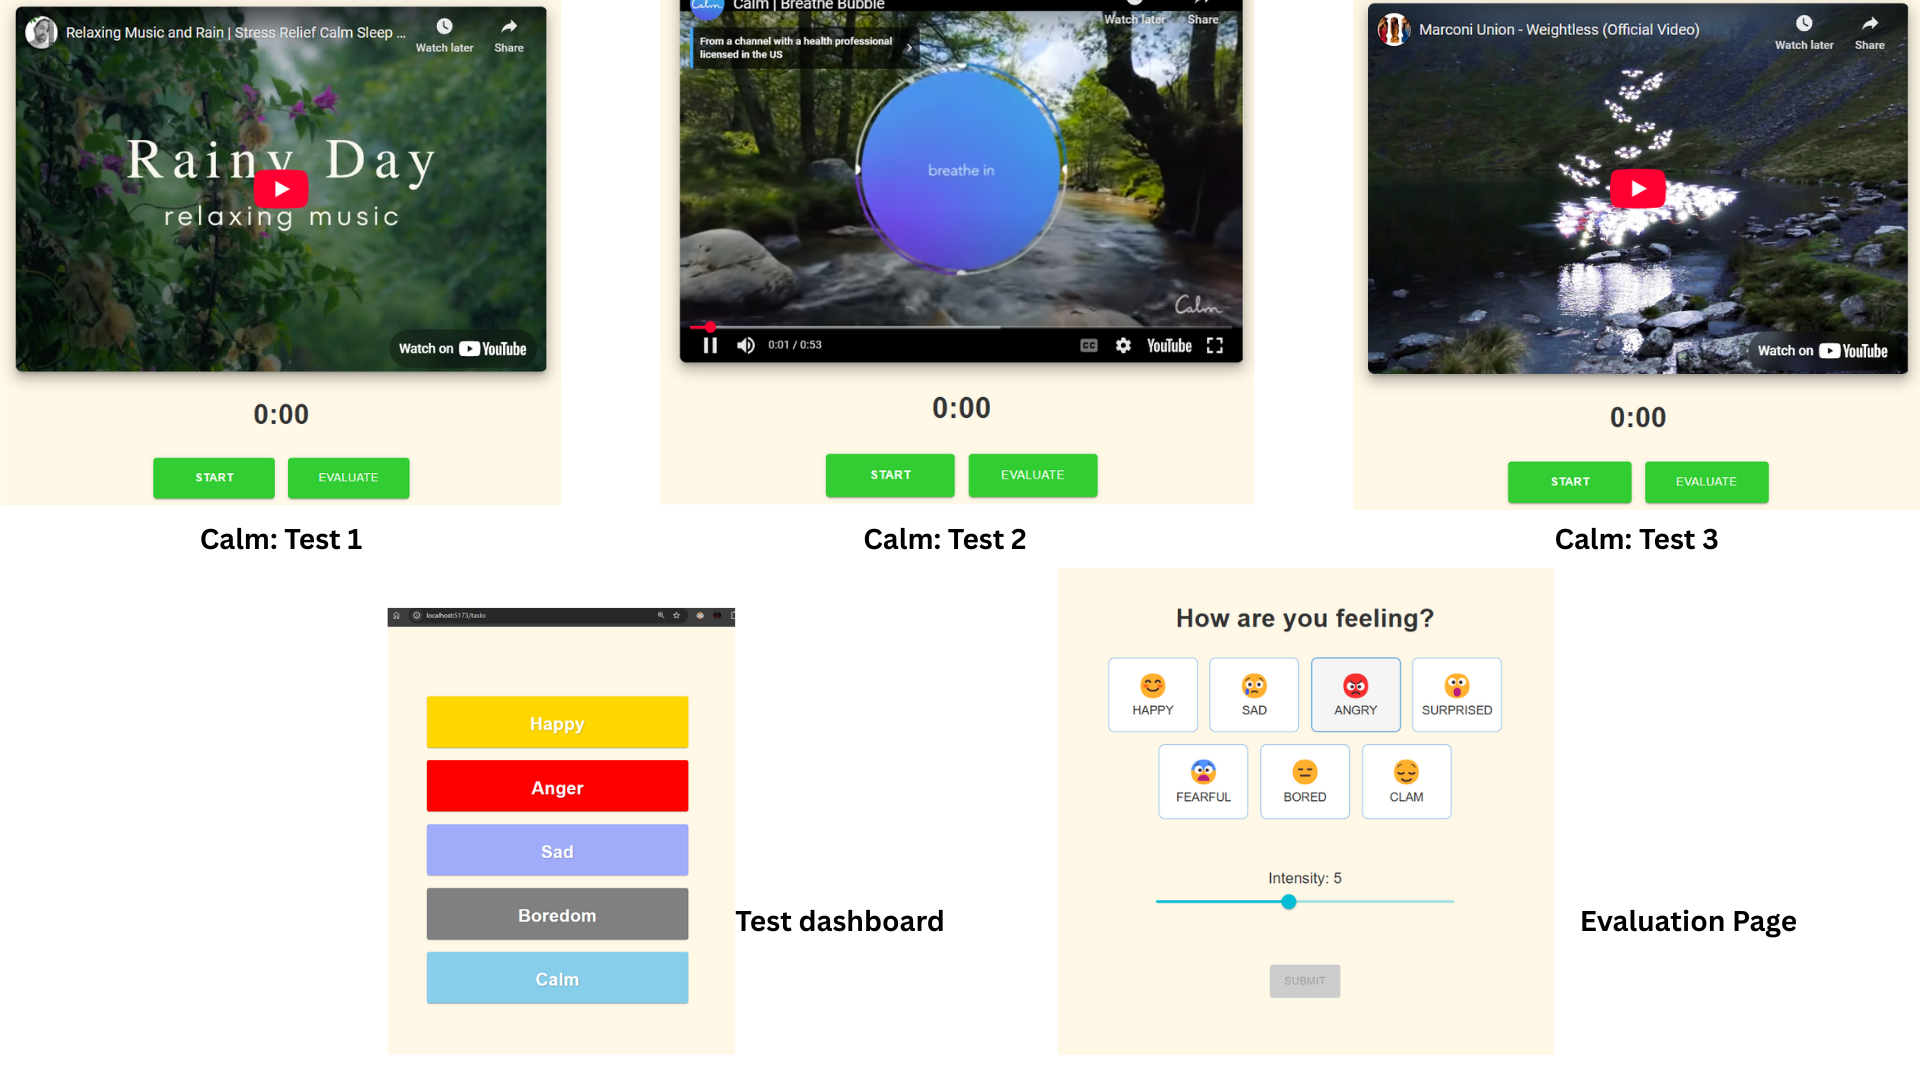
\includegraphics[width=1\textwidth]{img/chapter_03/calm_tests_eval.png}
    \caption{Screenshots from the three tasks used to elicit calmness and the evaluation page}
    \label{fig:calm_eval}
\end{figure*}

\begin{figure*}[h]
    \centering
    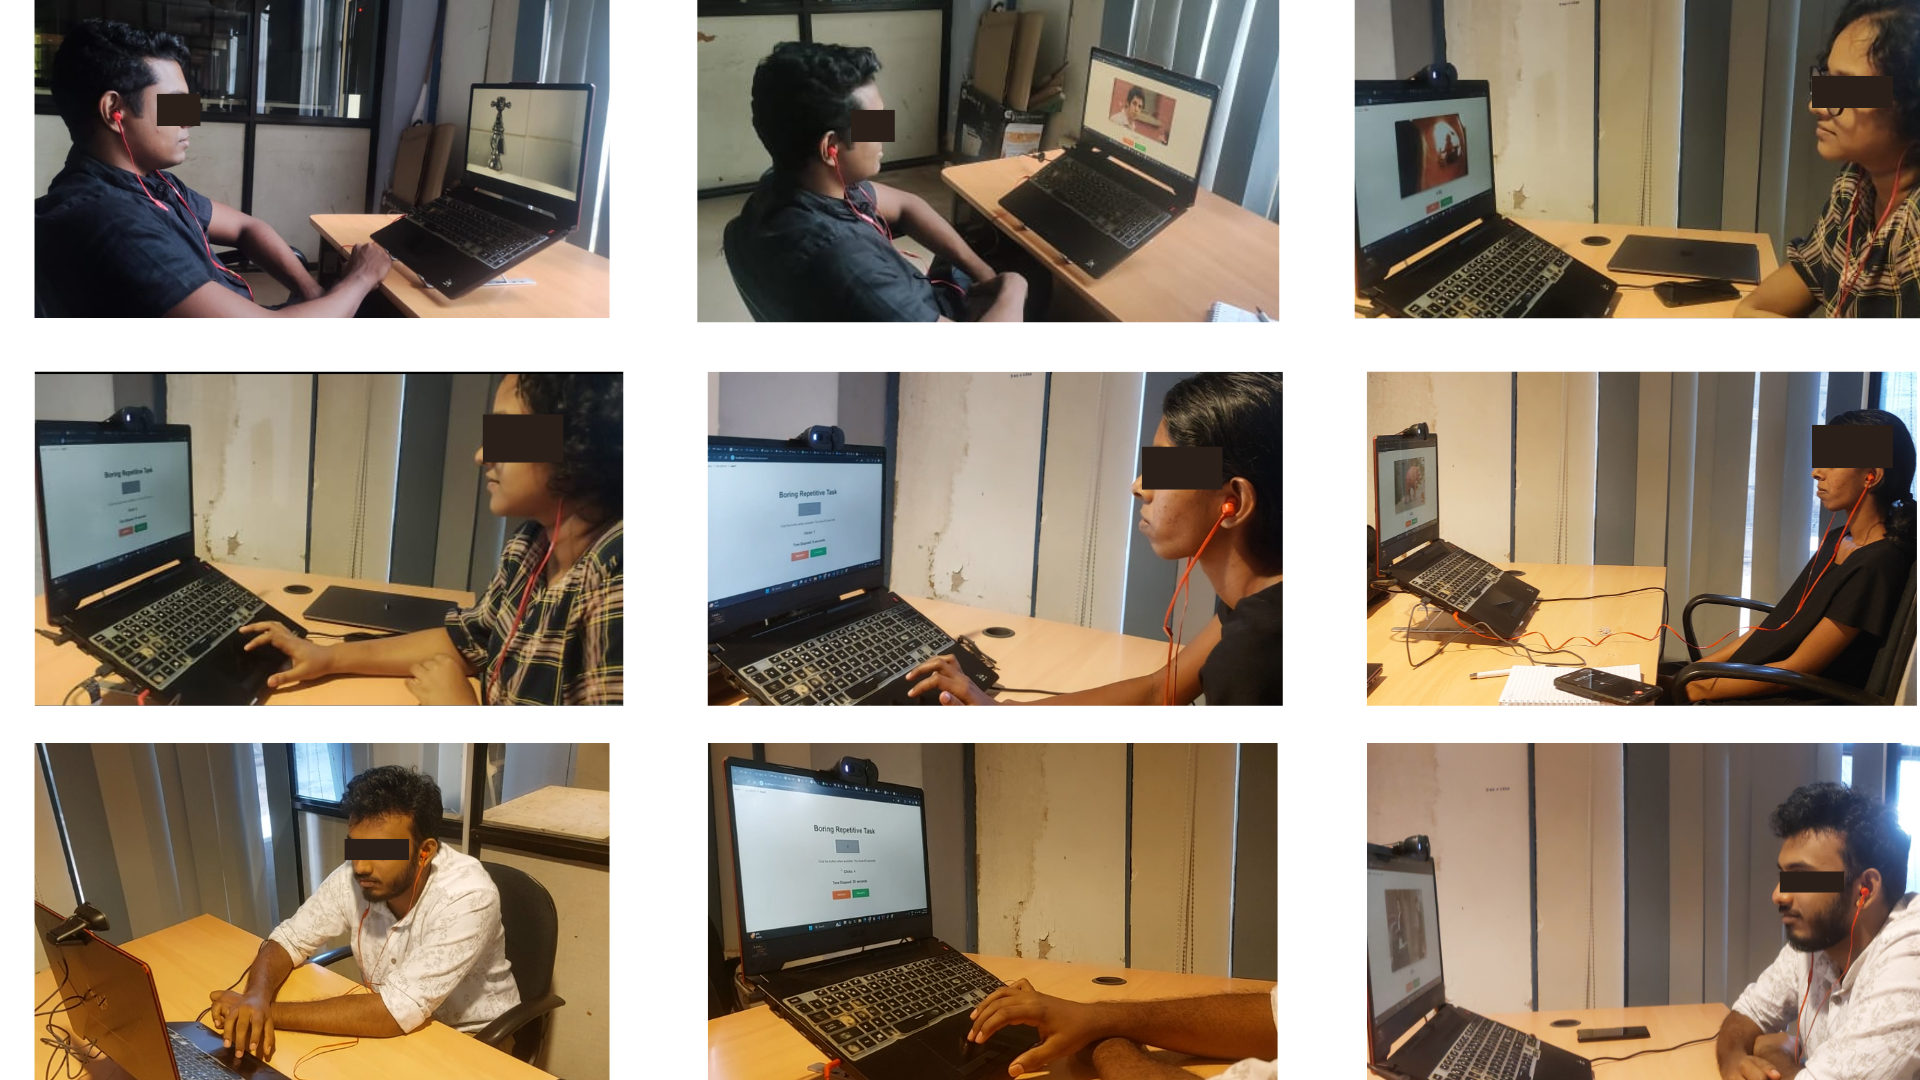
\includegraphics[width=1\textwidth]{img/chapter_03/participating.png}
    \caption{Snapshots of participants engaged in the emotion elicitation tasks.}
    \label{fig:participant_snapshots}
\end{figure*}

\begin{table}[h]
    \centering
    \caption{Summary of Emotion Eliciting Experiments}
    \label{tab:emotion_experiments}
    \begin{tabular}{|>{\raggedright\arraybackslash}p{2.5cm}|>{\raggedright\arraybackslash}p{2.5cm}|>{\raggedright\arraybackslash}p{4cm}|>{\raggedright\arraybackslash}p{5.5cm}|}
    \hline
    \textbf{Emotion} & \textbf{Intensity} & \textbf{Stimulus} & \textbf{Description} \\
    \hline
    \multirow{3}{*}{Happiness} 
    & Low & Funny prank video (\url{https://youtu.be/ZwJfXgTO7J4}) & Comedy video to induce mild amusement and smiling through light-hearted content \\
    \cline{2-4}
    & Medium & Autobiographical recall & Participants describe recent happy personal memory to invoke moderate happiness \\
    \cline{2-4}
    & High & Minesweeper game (high chance of winning) & Designed to trigger joy through accomplishment and reward feedback \\
    \hline
    
    \multirow{3}{*}{Anger} 
    & Low & Chrome Dino game + city noise (\url{https://youtu.be/d0k1JFAAMCo}) & Simple game with distracting honking sounds to create mild frustration \\
    \cline{2-4}
    & Medium & Number-clicking game + pop-ups + countdown & Ads and timers disrupt gameplay, increasing frustration and loss of control \\
    \cline{2-4}
    & High & Flappy Bird variant with broken controls & Unclear mechanics + noise designed to frustrate and break user expectation \\
    \hline
    
    \multirow{3}{*}{Sadness} 
    & Low & "Little Motel" song (\url{https://youtu.be/zqQTODR3kR8}) & Sad music with contextual explanation to invoke reflective sadness \\
    \cline{2-4}
    & Medium & Clip of young person in distress & Emotionally relatable video showing personal struggles and crying \\
    \cline{2-4}
    & High & "The Champ" (1979) death scene (\url{https://youtu.be/b5qwTeCj4jc}) & Highly validated emotional clip used to induce intense grief \\
    \hline
    
    \multirow{3}{*}{Boredom} 
    & Low & Button clicking task & Repetitive motor task with no variation or challenge \\
    \cline{2-4}
    & Medium & Dripping water video (\url{https://youtu.be/lVrYV0odeFY}) & Monotonous, slow-paced video with low informational content \\
    \cline{2-4}
    & High & Yawning video (\url{https://youtu.be/M3QYDtSbhrA}) & Triggers low arousal and disengagement, possibly contagious yawning \\
    \hline
    
    \multirow{3}{*}{Calmness} 
    & Low & Rain + relaxing music (\url{https://youtu.be/PjUZbgZfMOo}) & Gentle visuals and soft ambient music for mild relaxation \\
    \cline{2-4}
    & Medium & Relaxing music + breathing (\url{https://youtu.be/uxayUBd6T7M}) & Guided breathing exercise synchronized with music to enhance calm \\
    \cline{2-4}
    & High & "Weightless"(\url{https://youtu.be/UfcAVejslrU}) & Scientifically validated song with strong calming effect \\
    \hline
    \end{tabular}
\end{table}

\FloatBarrier%